\documentclass[11pt,a4paper,oldfontcommands,twosided,article]{memoir}
% Packages
\usepackage[utf8]{inputenc}
\usepackage[danish]{babel}
\usepackage [T1]{fontenc}
\usepackage[margin=2.5cm]{geometry}
\usepackage{amsmath}
\usepackage{color,colortbl}
\usepackage{amsfonts}
\usepackage{amssymb}
\usepackage{graphicx}
\usepackage{appendix}
\usepackage{listings}
\usepackage[font=it, labelfont=bf]{caption}
%\usepackage[protrusion=true,expansion=true]{microtype}
\usepackage{listings}
\usepackage{float}
\usepackage{color}
\newcommand*\mystrut[1]{\vrule width0pt height0pt depth#1\relax}
\renewcommand*{\appendixname}{Appendix}
\title{Korrespondance analyse af markbilleder}
\author{Christoffer Thrysøe, Andreas Borgstad}
\date{} % set date
\begin{document}
\maketitle % Insert title etc.
\pagenumbering{roman}
\newpage
\renewcommand{\contentsname}{Indholdsfortegnelse}
\setcounter{secnumdepth}{3}
\setcounter{tocdepth}{1}
\tableofcontents*
\newpage
\pagenumbering{arabic}
\chapter{Abstract} \label{sec:abstract}
\begin{center}
\textbf{Resumé}
\end{center}
Korrespondanceanalyse af markbilleder er et led i en process, hvis hovedformål er at relatere placering af ukrudt i markbilleder, til GPS koordinater. Korrespondanceanalysen består i at detektere punkter i billedet, knytte deskriptorer til disse og derefter matche punkterne. Fire forskellige detektorer (Difference og Gaussian, Determinant of Hessian, Harris og Morvec), samt to deskriptorer(SIFT og SURF) og en matching algoritme er beskrevet og implementeret. Determinant of Hessian og SURF, har givet den bedste repeatibility measure med en middelværdi 0.15063, for 10 billeder, på samme højde, hvor Harris og SIFT har givet andenbedste, med middelværdi på 0.1505. Det er konkluderet, at både hjørnedetektorer og blobdetektorer, kan bruges til at skabe korrespondancer.
\begin{center}
\textbf{Abstract}
\end{center}
Correspondanceanalysis of crop field images, is a part of a progress in which the main purpose is to relate the location of weed in the individual crop field images GPS coordinates....
\newpage
% Input secions here
\chapter{Introduction} \label{sec:intro}
Future Cropping er et forsknings projekt, oprettet af Miljøstyrelsen, der i samarbejde med Datalogisk institut og institut for Plante- og Miljøvidenskab skal hjælpe landmænd i at automatisere detektion af ukrudt i marker. Projektet har til formål at nedsætte landbrugets brug af pesticider, ved hjælp af en drone \footnote{UAV (eng. unmanned aerial vehicle} udstyret med kamera og GPS. Dronen tager et antal overlappende luft billeder over landmandens mark, disse billeder bliver analyseret og omdannet til et ukrudtskort, tilknyttet GPS koordinater.
Dette ukrudtskort behandles af en algoritme, der identificere præcis, hvor ukrudtet befinder sig og derved, hvor der er behov for pesticider\cite{drone}.
\section{Opgavens problemfelt} \label{subsec:felt}
Opgavens afsæt i dette projekt er bestemmelsen af, hvordan de individuelle billeder passer sammen, hvilket er det første skridt i etableringen af et ukrudtskort. Dette udføres ved at etablere korrespondancer imellem billederne taget af dronen, hvilket er muligt da billederne overlapper hinanden. Denne teknik vil refereres til som "korrespondance analyse". Korrespondance analyse er en billedebehandlings teknik, indenfor "computer vision" og består af følgende trin. (\textit{1}) Distinktive punkter detekteres i billederne som resultat af at anvende af en række matematiske modeller på billederne. Formålet ved dette stadie er udvælge de samme punkter/objekter i de overlappende billeder. (\textit{2}) Området omkring disse fundne punkter beskrives af en deskriptor. (\textit{3}) Hver deskriptor sammenlignes med andre fundne interessepunkter i andre billeder for at "matche" punkterne.
\section{Problemformulering} \label{subsec:form}
Med udgangspunkt i litteraturen inden for
korrespondanceanalyse samt implementering af
flere eksisterende metoder, hvilke metoder, teoretisk og praktisk, anvendes bedst til korrespondanceanalyse af markbilleder? \\ \\
\textbf{Udvidelse af problemformuleringen} \\
Der opstilles en beskrivelse af et udsnit af forskellige udvalgte metoder, der bliver brugt i feature detektion, feature deskription og matching. Der vil foretages korrespondanceanalyse af markbilleder, ved implementering af udvalgte eksisterende metoder. \\
Det eksperimentelle fokus i opgaven vil ligge på afprøvning af de forskellige metoder på markbilleder. Markbillederne har få distinktive træk, hvilket er egenskaber, der er vigtigt for korrespondance analyse. Udvælgelsen af metoder er baseret på hypoteser  ift. hvordan metoderne forventes at reagere på markbilleder. 
<not done, empririsk>
\\ \\
Markbilledernes manglende diversitet, samt inkonsistente forhold under fotograferingen diskuteret i [ref til afsnit om markbillederne], præsenterer nogle potentielle udfordringer ved korrespondanceanalysen. Udfordringerne gør det derfor interessant at undersøge, hvorvidt det er muligt at finde tilpas nok punkter, der kan anvendes. Hovedproblemet ved opgaven fokusere derfor på, hvordan der bedst kan detekteres features i markbillederne.
\subsection{Afgrænsning} \label{subsec:afg}
Projektet sigter på at afprøve allerede eksisterende metoder i et specifikt domæne og ikke
skabe nye metoder. Programmellet konstrueres mht. afklaring af de nævnte problemstillinger
og ikke mhp. efterfølgende at blive anvendt i praksis. De udvalgte metoder implementeres mhp. funktionaliteten, visse implementerings detaljer vil derfor undlades, hvis det enelige formål er at simplificere kompleksiteten.
\newpage
\chapter{Korrespondance Analyse} \label{sec:Kor}
Korrespondance problemet, imellem to eller flere billeder af samme objekt, referere til problemet om at finde et sæt af punkter i det ene billede, der kan identificeres og matches i det andet.
Udfordringen ved problemet ligger i at billederne, der skal matches, er udsat for en række ændringer, det kan f.eks. være forskydning i kameraets position ift. scenen eller  ændringer i scenens motiv. Et godt eksempel på korrespondance problemet er det menneskelige syn. Øjnene agere som to kameraer, der hver især fanger deres billede og omdanner disse billeder til ét sammenhængende panoramisk billede, ved hjælp af oprettelse af korrespondancer. Korrespondancen mellem øjnene tillader også opfattelse dybde i billedet, hvilket skyldes den horisontale forskydning af menneskets øjne. Denne sektion vil beskrive, hvordan denne korrespondance kan efterlignes af en computer.
\begin{figure}[H]
    \centering
    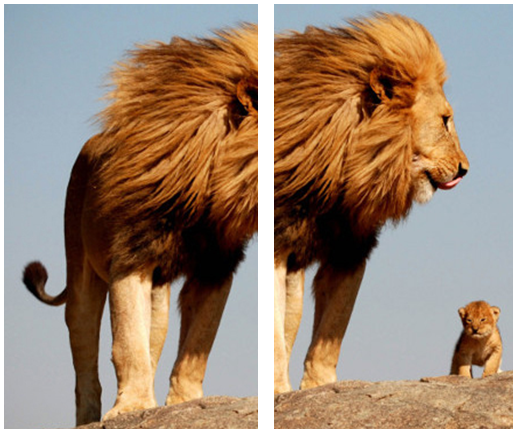
\includegraphics[width=0.45\textwidth]{fig/3.png}
     \vspace{-1em}
    \begin{center}    
       \caption{\textcolor{gray}{\footnotesize \textit{To billeder er af samme motiv, hvor kameraet fanger scenen fra to forskellige vinkler. F og F' angiver to korresponderende punkter, hvor den stiplede linje rammer de to scener \cite{kim}.}}}
    \label{fig:1}
     \end{center}
     \vspace{-2.5em}
  \end{figure} \noindent
I figur \ref{fig:1} ses to billeder af samme scene, men hvor kameravinklen er forskudt. For at opnå en korrespondance imellem billederne, skal der detekteres nogle unikke punkter, som optræder i begge billeder. I billedet er der udvalgt to korresponderende punkter \textit{F} og \textit{F'}. Disse punkter skal nøjes beskrives af en deskriptor \textit{D} så hvert punkt får tilknyttet en deskriptor $D(F)$ og $D(F')$. Det ønskes, for to korresponderende punkter, at: $D(F)\approx D(F')$, en nøje beskrivelse vil tillade korresponderende punkter at blive matched korrekt. Korrespondance analysens pipeline vil yderligere beskrives i denne sektion. Pipelinen består af følgende trin:
\begin{enumerate}
\item{Feature Detektion}
\item{Feature Deskription}
\item{Feature Matching}
\end{enumerate}
\section{Detektor}\label{sec:detect}
Feature detektion er en metode indenfor billedbehandling, der determinere, for hvert punkt i et billede (x,y), om dette punkt er et interessepunkt. Detektorens resultat vil derved være et subset af isolerede punkter fra billedet, der er markeret som interessante. (Så hvornår er punkter interessante?) Der er mange måder at definere hvad et interessepunkt er og i sidste ende bestemmer applikationsdomænet, hvilke punkter, der lokaliseres bedst. Interessepunkter kan f.eks. være kanter eller linjer i landskabet, ved genkendelse af veje fra satellitbilleder. Uanset hvilke strukturer, der ledes efter skal en detektor besidde følgende egenskaber:
\begin{itemize}
\item{\emph{Repeterbar}: Moravec \cite{moravec} definere et godt interessepunkt som værende et punkt, der entydigt kan lokaliseres i billeder, taget fra forskellige vinkler af en scene. Repeterbarheden significere detektorens uafhængighed af forskellige betingelser i billedet, dvs. dens evne til at detektere ens punkter i billeder, udsat for forskellige ændringer. }
\item{\emph{Distinktive:}
De fundne interessepunker skal være unikke ift. intensitetsvariationen i det omkringliggende område. Dette muliggør bedere beskrivelse af punktet og derved større mulighed for korrekt match.}
\end{itemize}
Ovenstående egenskaber kan opnås ved at tage højde for de ændringer, der kan forekomme i billederne, og derved være invariante overfor disse. Ændringerne kan være geometriske f.eks. rotation, skalering (se figur \ref{fig:skal}) eller affine transformationer. Det kan også være fotometriske ændringer i form af intensitetsskift i billederne forsaget af lysændringer.
\begin{figure}[H]
    \centering
    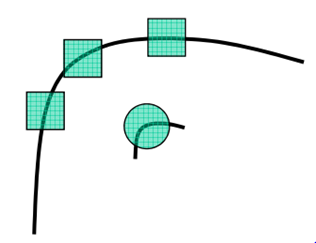
\includegraphics[width=0.37\textwidth]{fig/28.png}
     \vspace{-1em}
    \begin{center}    
       \caption{\textcolor{gray}{\footnotesize \textit{Figuren viser to ens kurver, der er set fra forskellige skalaer. Opfattes kurven langt væk fra, som den store kurve, vil de udvalgte områder opfattes som kanter. Skalere man ind på kurven vil området vise et hjørne. Det kan derfor, alt efter applikationsdomænet, være nødvendigt at anvende en skala invariant detektor.}}}
    \label{fig:skal}
     \end{center}
     \vspace{-2.5em}
  \end{figure} \noindent
Detektoren skal også være robust overfor små deformationer som støj i billedet, hvilket fejlagtigt kan fortolkes som interessepunkter. Interessepunkter defineres ikke udefra semantiske meningsfulde områder, som ansigter eller objekter, da dette vil kræve en høj-niveau fortolkning af scenen. I stedet anvendes lav-niveau strukturere, der identificeres i lokale pixel områder, som er matematisk definerbare og distinktive. Nedenstående er en gennemgang af forskellige lokale lav-niveau strukturere, der kan bruges i udvælgelsen af interessepunkter.
 \subsection{Hjørner}\label{subsec:corner}
En hjørnedetektor, leder efter hjørner i billedet og anvender disse som interessepunkter. Et hjørne kan defineres ved et punkt der har to dominerende kanter i hver sin retning.
\begin{figure}[H]
    \centering
    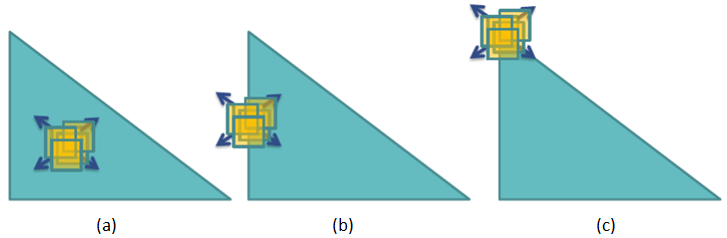
\includegraphics[width=0.55\textwidth]{fig/6.png}
    \vspace{-1em}   
    \begin{center}    
    \caption{\textcolor{gray}{\footnotesize \textit{
     Tre udvalgte vinduer, med interessepunkter i centrum af samme motiv. \textbf{(a)} Punktet er lokaliseret i en teksturløs region, d.v.s. ingen teksturskift. \textbf{(b)} Punktet er lokaliseret på en kant. \textbf{(c)} Punktet er lokaliseret på et hjørne }}}
    \label{fig:2}
     \end{center}
    \vspace{-2.7em}  
  \end{figure}  
\noindent
Hvorfor er hjørner gode punkter? Et hjørne er et godt interessepunkt da der foregår store intensitetsskift omkring hjørnets omliggende område og er derfor distinkt ift. området.
En intuitiv måde at definere hvorfor et punkt er interessant, er at placere et rektangulært vindue omkring punktet. Dette vindue forskydes lokalt i x og y retningen. Opstår der et nyt objekt, identisk med interessepunktet, som resultat af forskydningen af vinduet er punktet ikke lokalt distinkt. I figur \ref{fig:2} ses tre udvalgte punkter med et rektangulært vindue placeret over. I stil med ovenstående definition, forskydes det firkantede vindue i alle retninger. Forskydes \textbf{(a)} vil det matche alle de forskudte billeder da punktet og regionen omkring punktet er homogent. Punktet er derfor ikke distinkt. Forskydes \textbf{(b)} i x-aksen opnås et nyt objekt, men en forskydning i y-aksen vil resultere i samme objekt af en kant, og punktet er derfor ikke distinkt. Punktet placeret på et hjørne \textbf{(c)} er distinkt da ingen forskydninger vil matche original billedet. Hjørnet kan derfor bruges som et interessepunkt. At detektere hjørner er en udbredt teknik, da de er lokalt definerbare og ofte forekommer i forskellige scener.
\subsection{Kanter}\label{subsec:kant}
Som nævnt er kanter ikke lokalt distinkte, men kan bruges til at fjerne en del unødvendig information fra et billedet, ved kun at udtrykke kanterne.  En kant kan defineres som et skarpt skift i billedintensiteten. 
En måde at visualisere denne definition af en kant, er ved at opfatte billedet som en funktion, der afbilder billedintensiteten i 1-dimension. En høj kurve, angiver et skarpt intensitetsskift og derved en kant. Kanter kan derved identificeres ved at finde disse skarpe sving i intensitetsfunktionen, se figur \ref{fig:kant}.
\noindent
\begin{figure}[H]
    \centering
    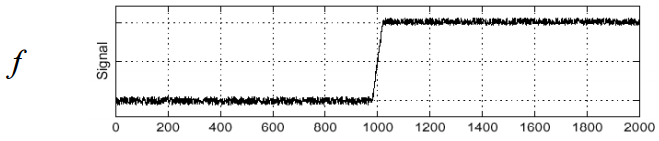
\includegraphics[width=0.55\textwidth]{fig/7.png}
     \vspace{-1em}
    \begin{center}        
     \caption{\textcolor{gray}{\footnotesize \textit{
     En 1-dimensional fortolkning af intensiteten i et billede. De små udsving indikere støj, den store kurve repræsenter et skrapt skift i intensiteten og derved en kant i et billedet.}}}
    \label{fig:kant}
     \end{center}
       \vspace{-2.5em}
  \end{figure}
\noindent
En differentiering af funktionen vil angive, hvor skarp kurven er og derved fremhæve dens udsving. Et 2-dimensionelt billede er ikke en kontinuerlig funktion, men består af diskrete værdier i form af pixel informationer.
Billedet differentieres derfor ved en approksimeret differentiering. Differentiering af en funktion \emph{f(x)} kan approksimeres til følgende diskrete differentiering:
\begin{equation}
\dfrac{df(x)}{dx}=\dfrac{f(x+1)-f(x-1)}{2}
\label{diff}
\end{equation}
Ovenstående i kan opnås ved at folde billedet med kernen $[1 \hspace{0.5cm} 0 \hspace{0.5cm} -1]$, hvor foldning af et billede \emph{I}, med en kerne \emph{K}: $I\oplus K$, hvor K har indgangen m x n og I M x N udregnes som:
\begin{equation}
O(i,j) = \sum\limits_{k=1}^m \sum\limits_{l=1}^m I(i+k-1,l-1)K(k,l)
\end{equation}
Hvor $O(i,j)$ er det nye punkt i billedet. Ved differentiering fremhæves udsving i intensitetsskiftene i billederne, hvilket gør det muligt at identificere kanterne. Problemet ved dette, visualiseret i figur \ref{fig:kant}, er at støj i billedet (de små udsving) også vil blive fremhævet, hvilket vil resultere i fejlagtige detektioner af kanter. For at imødekomme dette foldes billedet med et Gaussisk filter, hvilket er en approksimering til den Gaussiske funktion. Det Gaussiske filter kan bruges, i billedbehandling, til at beskrive et punkt, ved en vægtet normalfordeling i de omliggende pixel, visualiseret som en klokke, der ligges over billedet. Foldningen med et Gaussisk filter vil derfor resultere i en "flydende" overgang mellem pixel værdierne og derfor glatte billedet.  Den Gaussiske funktion i 2-D, hvor $ \sigma $ er standart afvigelsen, der angiver graden af glatningen, er defineret som:
\begin{equation}
G(x,y) = \frac{1}{2 \pi \sigma ^{2}} e^{- \frac{x^{2} + y^{2}}{2 \sigma ^{2}}}
\label{2dgaussian}
\end{equation} 
For at undgå itereration af biledet to gange, for differentiering og sløring, kan dette udføres i en samlet operation, ved at folde billedet med et differentieret Gaussisk filter, da foldning er en associativ operation. Yderligere, for at detektere kanter, kan denne operation udvides. Ved en differentiering bliver signalet fra figur ref til en kurve der ligner et bjerg. For en mere præcis definition af en kant, kan den dobbelt afledte tages som set i figur \ref{fig:deriv}.
\begin{figure}[H]
    \centering
    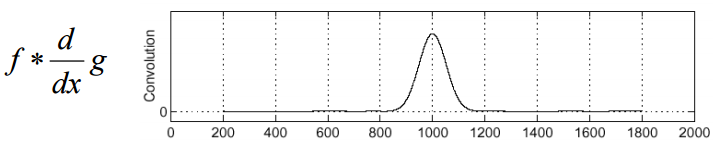
\includegraphics[width=0.55\textwidth]{fig/8.png}
    \vspace{-1em}   
    \begin{center}
    \caption{\textcolor{gray}{\footnotesize \textit{
     Resultatet af at folde et dobbelt differentieret Gaussisk filter med funktionen}}}
    \label{fig:deriv}
     \end{center}
    \vspace{-2.5em}  
  \end{figure}
\noindent
Kanten er nu let definerbar ved at lokalisere når funktionen krydser nul. I et 2-dimensionelt billede repræsentere intensitetsskift også en orientering. Vertikale kanter findes ved at folde billedet med et Gaussisk filter, differentieret i x-aksen og y-aksen for horisontale kanter.
\subsection{Blobs}
En blob detektor detektere regioner i billedet, hvor der sker en ændring af billedets egenskaber, det kan f.eks. være lysintensiteten ift. den omliggende region. En blob består af et sæt sammenhængnede pixels alle af samme intensitet, der er distinktive ift. området. Lindenberg \cite{blob} definere blobs som værende lyse regioner på sort baggrund eller omvendt, altså strukturer, der står i kontrast til deres baggrund. En blob kan derfor defineres som bestående af et område med \emph{mindst} ét lokalt ekstrema, enten et maksimum eller et minimum. Blobbens struktur er ikke semantisk intuitivt definerbar, men er matematisk veldefineret <?>.
\begin{figure}[H]
    \centering
    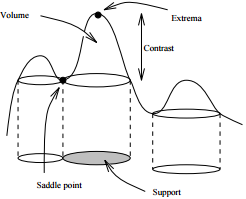
\includegraphics[width=0.35\textwidth]{fig/11.png}
    \vspace{-0.5em}   
    \begin{center}
    \caption{\textcolor{gray}{\footnotesize \textit{
    En blob visualiseret i 2-d, udefra Lindenberg's definition \cite{blob}}}}
    \label{fig:lindblob}
     \end{center}
  \end{figure}
       \vspace{-2.7em}
\noindent
I figur \ref{fig:lindblob}(a), ses en blob defineret af dets lokale ekstrema, hvor styrken af blobben beksrives ved kontrasten, ift. området omkring ekstremaet. Lindenberg definere blobbens domæne som værende afgrænset af dens "saddle point". Et "saddle point" angiver punktet, hvor intensiteten stopper med at falde og starter med at stige for lyse blobs, og modsat for mørke. Punktet definere altså, hvordan blobben er lokalt præsenteret. Denne definition på en blob stemmer overens med definitionen af interessepunkter. Det lokale ekstrema gør blobben til en veldefineret lokal struktur og derved distinktiv. Blobs har også en fordel ift. kant og hjørne detektion, da blobs indgår i de fleste domæner. Kanter og hjørner forekommer ofte i menneskeskabte scener, ved veldefinerede strukturer. Blobs har derfor flere applikationsområder, og kan bruges indenfor billeder af objekter, der ikke er menneskelige defineret scener, f.eks. indenfor medicinsk billedanalyse til detektion af anomalier i røntgenbilleder.  Ligesom i kant-detektion, kan blobs beskrives ved intensitetsskift, hvor der forekommer en krusning rundt om ekstremaet. En metode til at detektere disse ekstremaer hedder Laplacian operatoren: $\Delta^2$. Laplace operatoren anvendes på et gaussisk filter og opnår operatoren "Laplacian of Gaussian" \eqref{lap}:
\begin{equation}
\Delta^2 f = \dfrac{\partial^2 f}{\partial x^2}+\dfrac{\partial^2 f}{\partial y^2}, \Delta^2G_{\sigma}(x,y)
\label{lap}
\end{equation}
Laplacian of gaussian operatoren kan diskritiseres og og foldes med billedet for at finde lokale ekstremaer. Figur \ref{fig:lapgauss} viser, hvordan laplace operatoren opnår et maximum i centeret af en blob, og at blobben derved bliver lokaliserbar. Hvis blobben (b), er tyndere eller tykkere vil laplace operatoren ikke længere resultere i et ekstrema, men nærmere et kant respons. Det er derfor nødvendigt at normalisere laplace filteret ift. hvilken størrelse blobben har.
\begin{figure}[H]
    \centering
    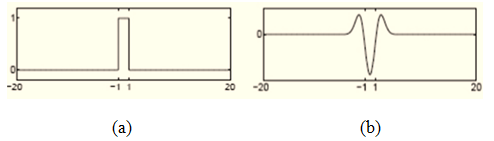
\includegraphics[width=0.60\textwidth]{fig/16.png}
    \vspace{-0.5em}   
    \begin{center}
    \caption{\textcolor{gray}{\footnotesize \textit{
    (a) En 3-D visualisering af en to-dimensional Laplacian of Guassian (b) ét en-dimensionalt signal (c) Laplacian of Gaussian operatoren anvendt på (b)}}}
    \label{fig:lapgauss}
     \end{center}
  \end{figure}
       \vspace{-2.5em}
\noindent
Blobs forekommer, ligesom andre strukturer, på forskellige skalaer, bestemt af størrelsen af objektet og objektets placering i billedet. I figur \ref{fig:scale} angiver cirklerne den undersøgte skala, hver skala illustrere forskellige objekter. Skala invarians er nødvendigt, hvis der forekommer ændringer i skalaen imellem billederne, men også for at detektere blobs af forskellige størrelser.
\begin{figure}[H]
    \centering
    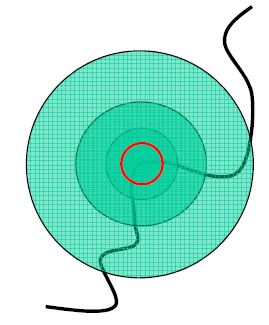
\includegraphics[width=0.25\textwidth]{fig/29.png}
    \vspace{-0.5em}   
    \begin{center}
    \caption{\textcolor{gray}{\footnotesize \textit{
    }}}
    \label{fig:scale}
     \end{center}
  \end{figure}
       \vspace{-2.5em}
\noindent
<hvordan dette gøres GOD>
Så hvordan udvælges cirklen, der dækker interesse området uafhængigt af områdets størrelse.  For Blobs er det interessant når der i et skaleret område opstår et ekstrema. En måde at søge efter ekstrema over forskellige skalaer er ved at oprette et skalarum for det undersøgte billede, hvor hvert billede skaleres og der for hver skala udvælges features. Skala-rummet i et 2-dimensionalt billede repræsenteres af flere billeder i forskellige skalaer af det originale billede. Billeder, der repræsentere forskellige skalaer, opnås ved at folde billedet med et 2-dimensionalt Gaussisk filter. 
\begin{figure}[H]
    \centering
    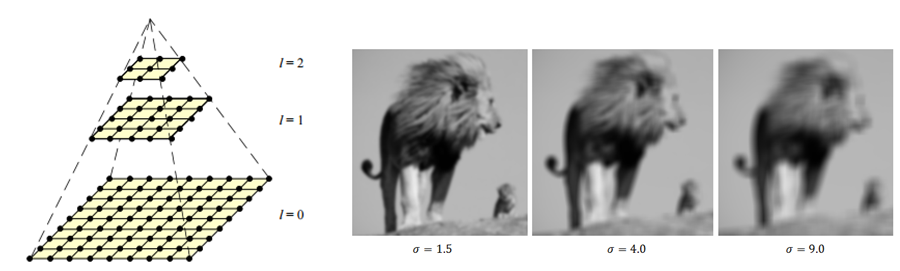
\includegraphics[width=0.65\textwidth]{fig/24.png}
    \vspace{-0.5em}   
    \begin{center}
    \caption{\textcolor{gray}{\footnotesize \textit{
Til venstre ses en visualisering af et skala-rum formet som en pyramide. Hvert niveau angiver en skala repræsentation af det originale vindue, hvor toppen af pyramiden indeholder billeder af største skala og derfor med mindst information, og bunden af skalaen med det originale billede. Til højre ses et billede foldet med et Gaussisk filter af stigende sigma værdier. Jo højere sigma værdi, jo flere fine detaljer bliver fjerne og billedet slørret.
    }}}
    \label{fig:mona}
     \end{center}
  \end{figure}
       \vspace{-2.5em}
\noindent
Iterativ Gaussisk slørring med stigende sigma værdier, bruges til at at generere et skalarum af billedet.
Et Gaussisk filter bruges da gradvis højere værdier af $\sigma$ fjerner fine strukturer, som vist i figur \ref{fig:mona} og nye objekter forekommer ikke ved transformationen fra finere til grovere skalaer \cite{lindenscale}. Idéen er derved at fjerne disse strukturer og, fremhæve andre objekter gradvist på en større skala der også kan detekteres.
Et billede i skalarummet for billedet $f(x,y)$ kan derfor defineres som i \eqref{scalespace}
\begin{equation}
L(x,y,\sigma) = g(x,y,\sigma)\ast f(x,y)
\label{scalespace}
\end{equation}
hvor $g$ er det 2-dimensionelle Gaussiske filter,$L(x,y,\sigma)$ repræsentere et et billede i skala-rummet, og skala-parametren $\sigma$, bestemmer skalaen, eller placeringen i skala-rummet. $L(x,y,0) = f(x,y)$, da det er den "nederste" skala og den nederste del af pyramiden. Højere niveauer af pyramiden kan opnås ved at folde billedet med et Gaussisk filter af større sigma værdi.
\section{Deskriptor}
For at udvælge korresponderende punkter imellem billederne, skal interessepunkterne beskrives af en deskriptor $Des$. Deskriptoren er en funktion, der tager et billede og et punkt som input og returnerer en feature. Deskriptoren beskriver et interessepunkt ud fra information i og omkring punktet, og tilknytter punktet en feature $f$, i form af en n-dimensional vektor:
\begin{equation}
Des(I,p_i)=f_i
\end{equation}
\begin{equation}
Des(I',p_j')=f_j'
\end{equation}
For to korresponderende punkter $i$ og $j$ ønskes det at $f_i \approx f'_j$, så punkterne kan identificeres som værende korresponderende punkter, men også for to \textit{ikke} korresponderende punkter $k$ og $l$ at $f_k \not\approx f'_l$.
\section{Matching}
Når der er udvalgt et sæt interessepunkter og deres deskriptorer er oprettet, skal punkterne matches. Det er ikke alle fundne punkter, der har et korresponderende punkt i det modsvarende billede alt afhængigt af transformatione, overlap og okklusion i billedet. For hvert udvundet interessepunkt er der en tilhørende x-dimensional vektor, oprettet af deskriptoren, der beskriver interessepunktet udefra en given information. Denne vektor skal sammenlignes mede vektorer i det modsvarende billede, for at finde det bedste match. Det "bedste match" kan kvantificeres til at være den vektor, der har den mindste Euklidiske afstand \eqref{euc} til det undersøgte interessepunkt. 
\begin{equation}
||P|| = \sqrt{\sum\limits_{i=1}^n(q_i-p_i)^2}
\label{euc}
\end{equation}
Om to euklidiske afstande angiver et match kan defineres ved at sætte en sætte en grænseværdi. Der er dog visse problemer ved at sætte en sådan grænseværdi. Sættes den for lavt opstår falske negative match og sættes den for højt opstår der falske positive match se figur \ref{fig:skift}. Forskellige transformationer i billedet kan også gøre at de målte afstande ligger længere væk end normalt eller omvendt, det er derved usikkert at definere en generel grænseværdi. En anden anvendelig metode er at matche med den "nærmeste nabo", hvor hvert punkt bliver matchet med det nærmeste (euklidiske) punkt. Her vil der også typisk sættes en grænseværdi for at fravælge dårligt defineret korrespondancer. Dette kan dog også være et problem i visse applikation, hvor nogle punkter matcher flere punkter.
\begin{figure}[H]
    \centering
    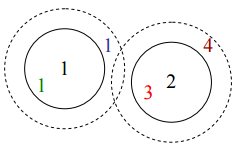
\includegraphics[width=0.35\textwidth]{fig/22.png}
    \vspace{-0.5em}   
    \begin{center}
    \caption{\textcolor{gray}{\footnotesize \textit{Problemet ved at sætte en grænseværdi: De sorte tal 1$\&$2 er features der skal matches mod et sæt andre features. Den solide inderste cirkel definere  en grænseværdi. Det grønne {\color{OliveGreen}1} er en sand positiv, det blå {\color{blue}1} er en falsk negativ(skulle havde været positiv), det røde {\color{red}3} er en falsk positiv (forkert vurderet). Sættes grænseværdien højere (til den stiplede linje) bliver det blå {\color{blue}1} en sand positiv, men den røde {\color{BrickRed} 4} bliver en falsk positiv. \cite{book1}}}}
    \label{fig:skift}
     \end{center}
  \end{figure}
       \vspace{-2.5em}
\noindent
Yderligere kan den "nærmeste-nabo" \textit{NN}\footnote{Nearest Neighbor}metode udvides til at kigge på den næst-nærmeste-nabo \textit{NNDR}\footnote{Nearest Neighbour Distance Ratio} ift. den "nærmeste-nabo", en metode introduceret i \cite{eval}.
\begin{equation}
N\!N\!D\!R=\dfrac{d_1}{d_2}=\dfrac{||D_A-D_B||}{||D_A-D_C|}
\label{nndr}
\end{equation}
hvor $d_1$ er den nærmeste-nabo distance og $d_2$ er den næst-nærmeste-nabo distance, $D_A$ er den udvalgte deskriptor, $D_B$ og $D_C$ er de to nærmeste naboer. Fordelen ved at anvende \eqref{nndr} ift. nærmeste-nabo, er at den straffer matches, der har en tæt euklidisk afstand med den næst-nærmeste nabo. Dette er fordelagtigt i visse sammenhæng f.eks. hvis man har nogle punkter, der matcher mange andre punkter, hvor man gerne vil have de distinktive matches, der kun har ét tydeligt korresponderende punkt se figur \ref{fig:skift2}.
\begin{figure}[H]
    \centering
    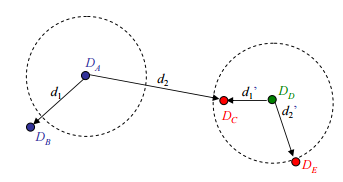
\includegraphics[width=0.35\textwidth]{fig/23.png}
    \vspace{-0.5em}   
    \begin{center}
    \caption{\textcolor{gray}{\footnotesize \textit{
      Matching med grænseværdi,\textit{NN} og \textit{NNDR} matching:
       Anvendes en simpel grænseværdi (stiplede linjer)  opstår der en falsk negativ med $D_A$ og $D_B$, $D_D$ matcher ukorrekt med $D_C$ og $D_E$    
       Anvendes metoden NN matcher $D_A$ korrekt $ D_B$, men matcher ukorrekt $D_D$ og $D_C$. Anvendes NNDR metoden matcher $D_A$ korrekt med $D_B$ og korrekt afviser match med $D_D$
     \cite{book1}}}}
    \label{fig:skift2}
     \end{center}
  \end{figure}
       \vspace{-2.5em}
\noindent
\newpage
\chapter{Analyse af markbilleder} \label{sec:mark}
Denne sektion har til formål at klarlægge udfordringer ved korrespondanceanalysen af markbilleder. Udfordringerne opstilles på baggrund af en undersøgelse af billederne og vil resultere i hypoteser om, hvilke egenskaber de korrespondanceanalytiske metoder skal besidde, for at muliggøre en korrespondanceanalyse.
\section{Dronens flyverute}
Dronen får fire punkter, der svarer til markens fire hjørner. Dronen starter derefter i et hjørne og flyver systematisk fra side til side, med samme orientering, for at overflyve hele marken. Dronen starter på en højde af ca. 60 meter og foretager en overflyvning af marken, hvorefter den falder i højde og overflyver marken igen. Processen gentages tre gange, indtil dronen er omkring 5-10 meter over marken. 
%I det udvalgte billedsæt er der fire overflyvninger, hvor hver overflyvning foregår på nogenlunde samme højde.
\section{Markbilleder}
I denne opgave er et sæt billeder, fra samme overfløjede kornmark anvendt. På det udvalgte billedsæt ses en kornmark, der består af umiddelbare tilfældige kornstrukturer. I nogle billeder er der traktorspor, og delvist pløjede kornområder. I figur \eqref{fig:korn} ses tre udsnit af et markbillede. De forskellige udsnit er af relativ identisk udseende og det er derfor umiddelbart svært at udpege hvor i billedet, udsnittende er taget fra. Ligheden billederne og de a priori tilfældige kornstrukturer, kan derfor besværliggøre korrespondanceanalysen. De umiddelbare udfordringer gør det interessant at undersøge, hvorvidt det er muligt at opnå korrespondancer.
\begin{figure}[H]
    \centering
    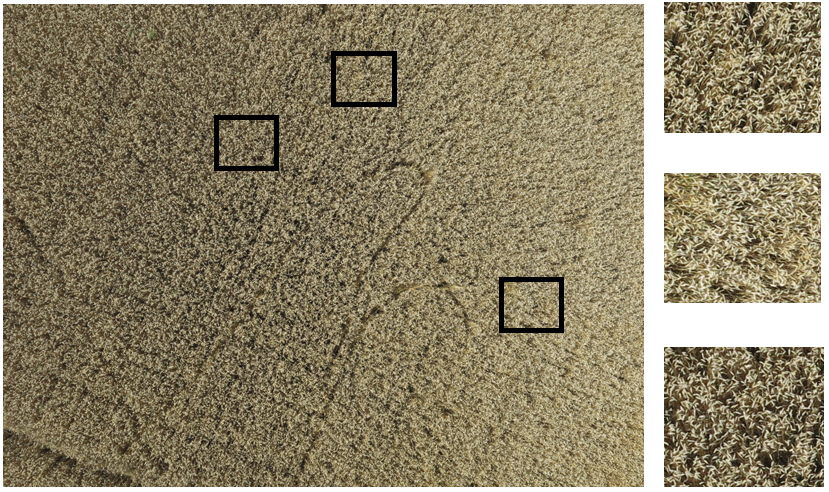
\includegraphics[width=0.85\textwidth]{fig/20a.png}
     %\vspace{-1em}
    \begin{center}    
       \caption{{\footnotesize \textit{Tre udsnit taget fra et markbillede.}}}
    \label{fig:korn}
     \end{center}
     \vspace{-2.5em}
  \end{figure} \noindent
Følgende observationer er gjort af markbillederne, samt forhold omkring overflyvningen:
\begin{itemize}
\item{\textbf{Overlap:} Overlappet imellem billederne har en signifikant indflydelse på korrespondanceanalysen. Et stort overlap vil betyde at interessepunkter har større sandsynlighed for at indgå i begge billeder. Derfor, ved mindre overlap, skal der udvælges flere interessepunkter. Det er bekræftet at billederne i gennemsnit overlapper hinanden med ca. 70\%. Overlappet afhænger af hvilken højde billederne er taget på - jo længere fra jorden billedet er taget, jo større er overlappet. Figur \ref{fig:overlap} viser fire billeder, sat sammen parvist, der er taget ved to forskellige højder, hvor billedernes overlap er markeret med blåt. (a) er taget når dronen er når dronen er længst fra jorden, billederne er estimeret til at overlappe hinanden med ca. 80 $\%$. (b) er taget ved en lavere højde, billederne overlapper hinanden med ca. 35$\%$.
\begin{figure}[H]
    \centering
    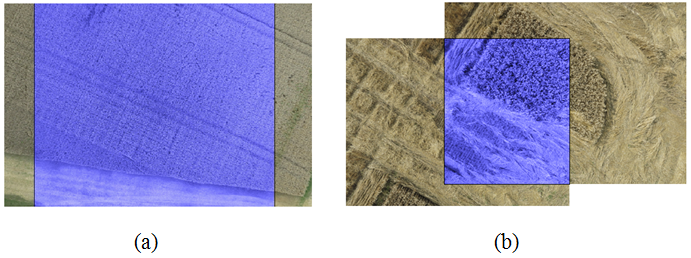
\includegraphics[width=0.85\textwidth]{fig/17.png}
     \vspace{-1em}
    \begin{center}    
       \caption{{\footnotesize \textit{Markbilleder taget ved forskellige højder, det blå område viser billedernes overlap.}}}
    \label{fig:overlap}
     \end{center}
     \vspace{-2.5em}
  \end{figure} \noindent }
\item{\textbf{Rotation:} Der er observeret mindre grad af rotation imellem billederne.
Den største grad af rotation er observeret i de to billeder, hvor dronen er nået kanten og skifter flyveretning. Denne rotation er registreret til at være 10-15$^{\circ}$ og er illustreret i figur \ref{fig:rotation}.
\begin{figure}[H]
    \centering
    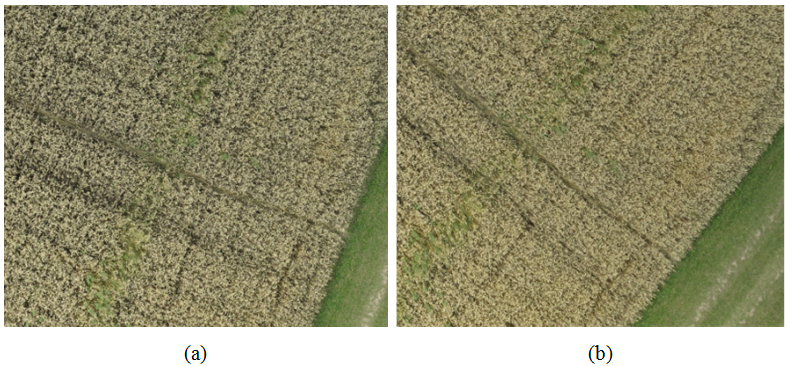
\includegraphics[width=0.85\textwidth]{fig/19.png}
     \vspace{-1em}
    \begin{center} 
       \caption{{\footnotesize \textit{Dronen skal til at ændre flyveretning, hvilket giver rotation imellem billederne.}}}
    \label{fig:rotation}
     \end{center}
     \vspace{-2.5em}
  \end{figure} \noindent}
\item{\textbf{Okklusion:}
I et cirkulært område, hvor kameraet står 90$^{\circ}$ på marken (ca. midten af billedet), vil jorden imellem kornet være mere synligt end i resten af markbilledet.
\begin{figure}[H]
    \centering
    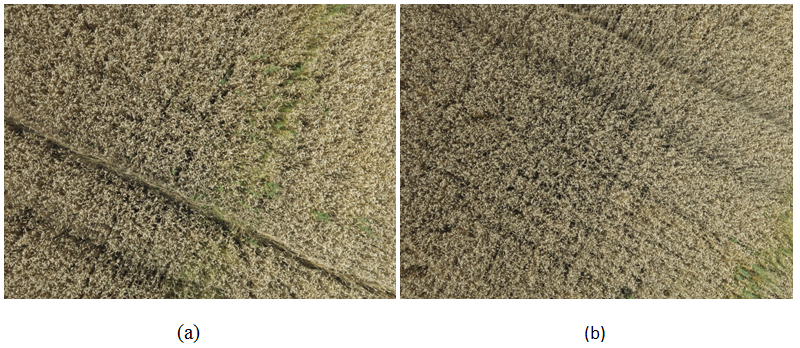
\includegraphics[width=0.85\textwidth]{fig/18.png}
     \vspace{-1em}
    \begin{center}    
       \caption{{\footnotesize \textit{ To forkudte billeder, hvor traktorsporet er okkluderet. }}}
    \label{fig:okklusion}
     \end{center}
     \vspace{-2.5em}
  \end{figure} \noindent
Figur \ref{fig:okklusion} er et eksempel på okklusion af jord, hvor (a) traktor spor optræder direkte under dronen og man kan derfor se jorden(b) derefter forskudt. Traktorsporet er ikke længere synlig.}
%\item{\textbf{Struktur} }
\end{itemize}
\section{Hypoteser}
Ud fra ovenstående analyse er der opstillet følgende hypoteser om krav til de udvalgte metoder:
\begin{itemize}
%\item{ <Det forventes, grundet strukturen af korn, at detektorer som leder efter veldefinerede strukturer, som hjørner, ikke vil have en god effekt på korn, men at blobs vil give bedre resultater.> }
\item{Det forventes ikke at metoderne behøver være invariante overfor rotation, grundet den lille rotation der forekommer imellem billederne.}
\item{Det forventes at metoderne skal være skalainvariante, da fotograferingen sker ved skiftende højde.}
\item{Jo tættere billederne er taget fra jorden, jo mindre er overlappet. Det forventes derfor, for billeder taget tæt på jorden, at detektoren skal tilpasses til at finde mange punkter, for at sikre en repeterbar detektion.}
\item{Det forventes ikke at der skal tages højde for problemer ved okklusion. Dog er graden af okklusion større, ved lavere højde, og dette kan have indflydelse på antallet af korrekte korrespondancer.
%Et overvejet tiltag var ikke at undersøge et område direkte under dronen, men det blev konkluderet at .
}
\item{Det forventes, grundet den umiddelbare tilfældige struktur i kornet, at hjørnedetektorer, ikke vil være i stand til at detektere korresponderende punkter.}
\end{itemize}
\newpage
% Litteraturliste
\bibliographystyle{abbrv}
\nocite{}
\bibliography{litterature}
\newpage
% Appendix
\appendix
\def\@chapapp{Appendix}
\chapter{Cost effectiveness Calculations} 
appendix test
\end{document}